\chapter{Preparazione al Testing}\label{ch:preparazione_testing}

\section{Configurazione dell'ambiente indoor}
La configurazione dell'ambiente consiste nella disposizione dei dispositivi Bluetooth nel modo corretto.
Per poter avere una ricezione dei segnali inviati dagli iBeacon senza troppi disturbi, questi devono essere così disposti:
\begin{itemize}
	\item su pareti regolari a circa 1 metro da terra;
	
	\item lontano da apparecchi che emettono onde elettromagnetiche (ad esempio router wifi);
	
	\item al sicuro da raffiche di vento;
	
	\item in aree in cui non si frappongano oggetti o persone tra lo smartphone e l'iBeacon target.
\end{itemize}

\newpage
\section{Collegamento Arduino-smartphone}

Come si può vedere nella Fig. \ref{fig:collegamento_Arduino-smartphone} viene indicato il collegamento diretto Arduino-smartphone
\begin{figure}[ph]
	\centering
	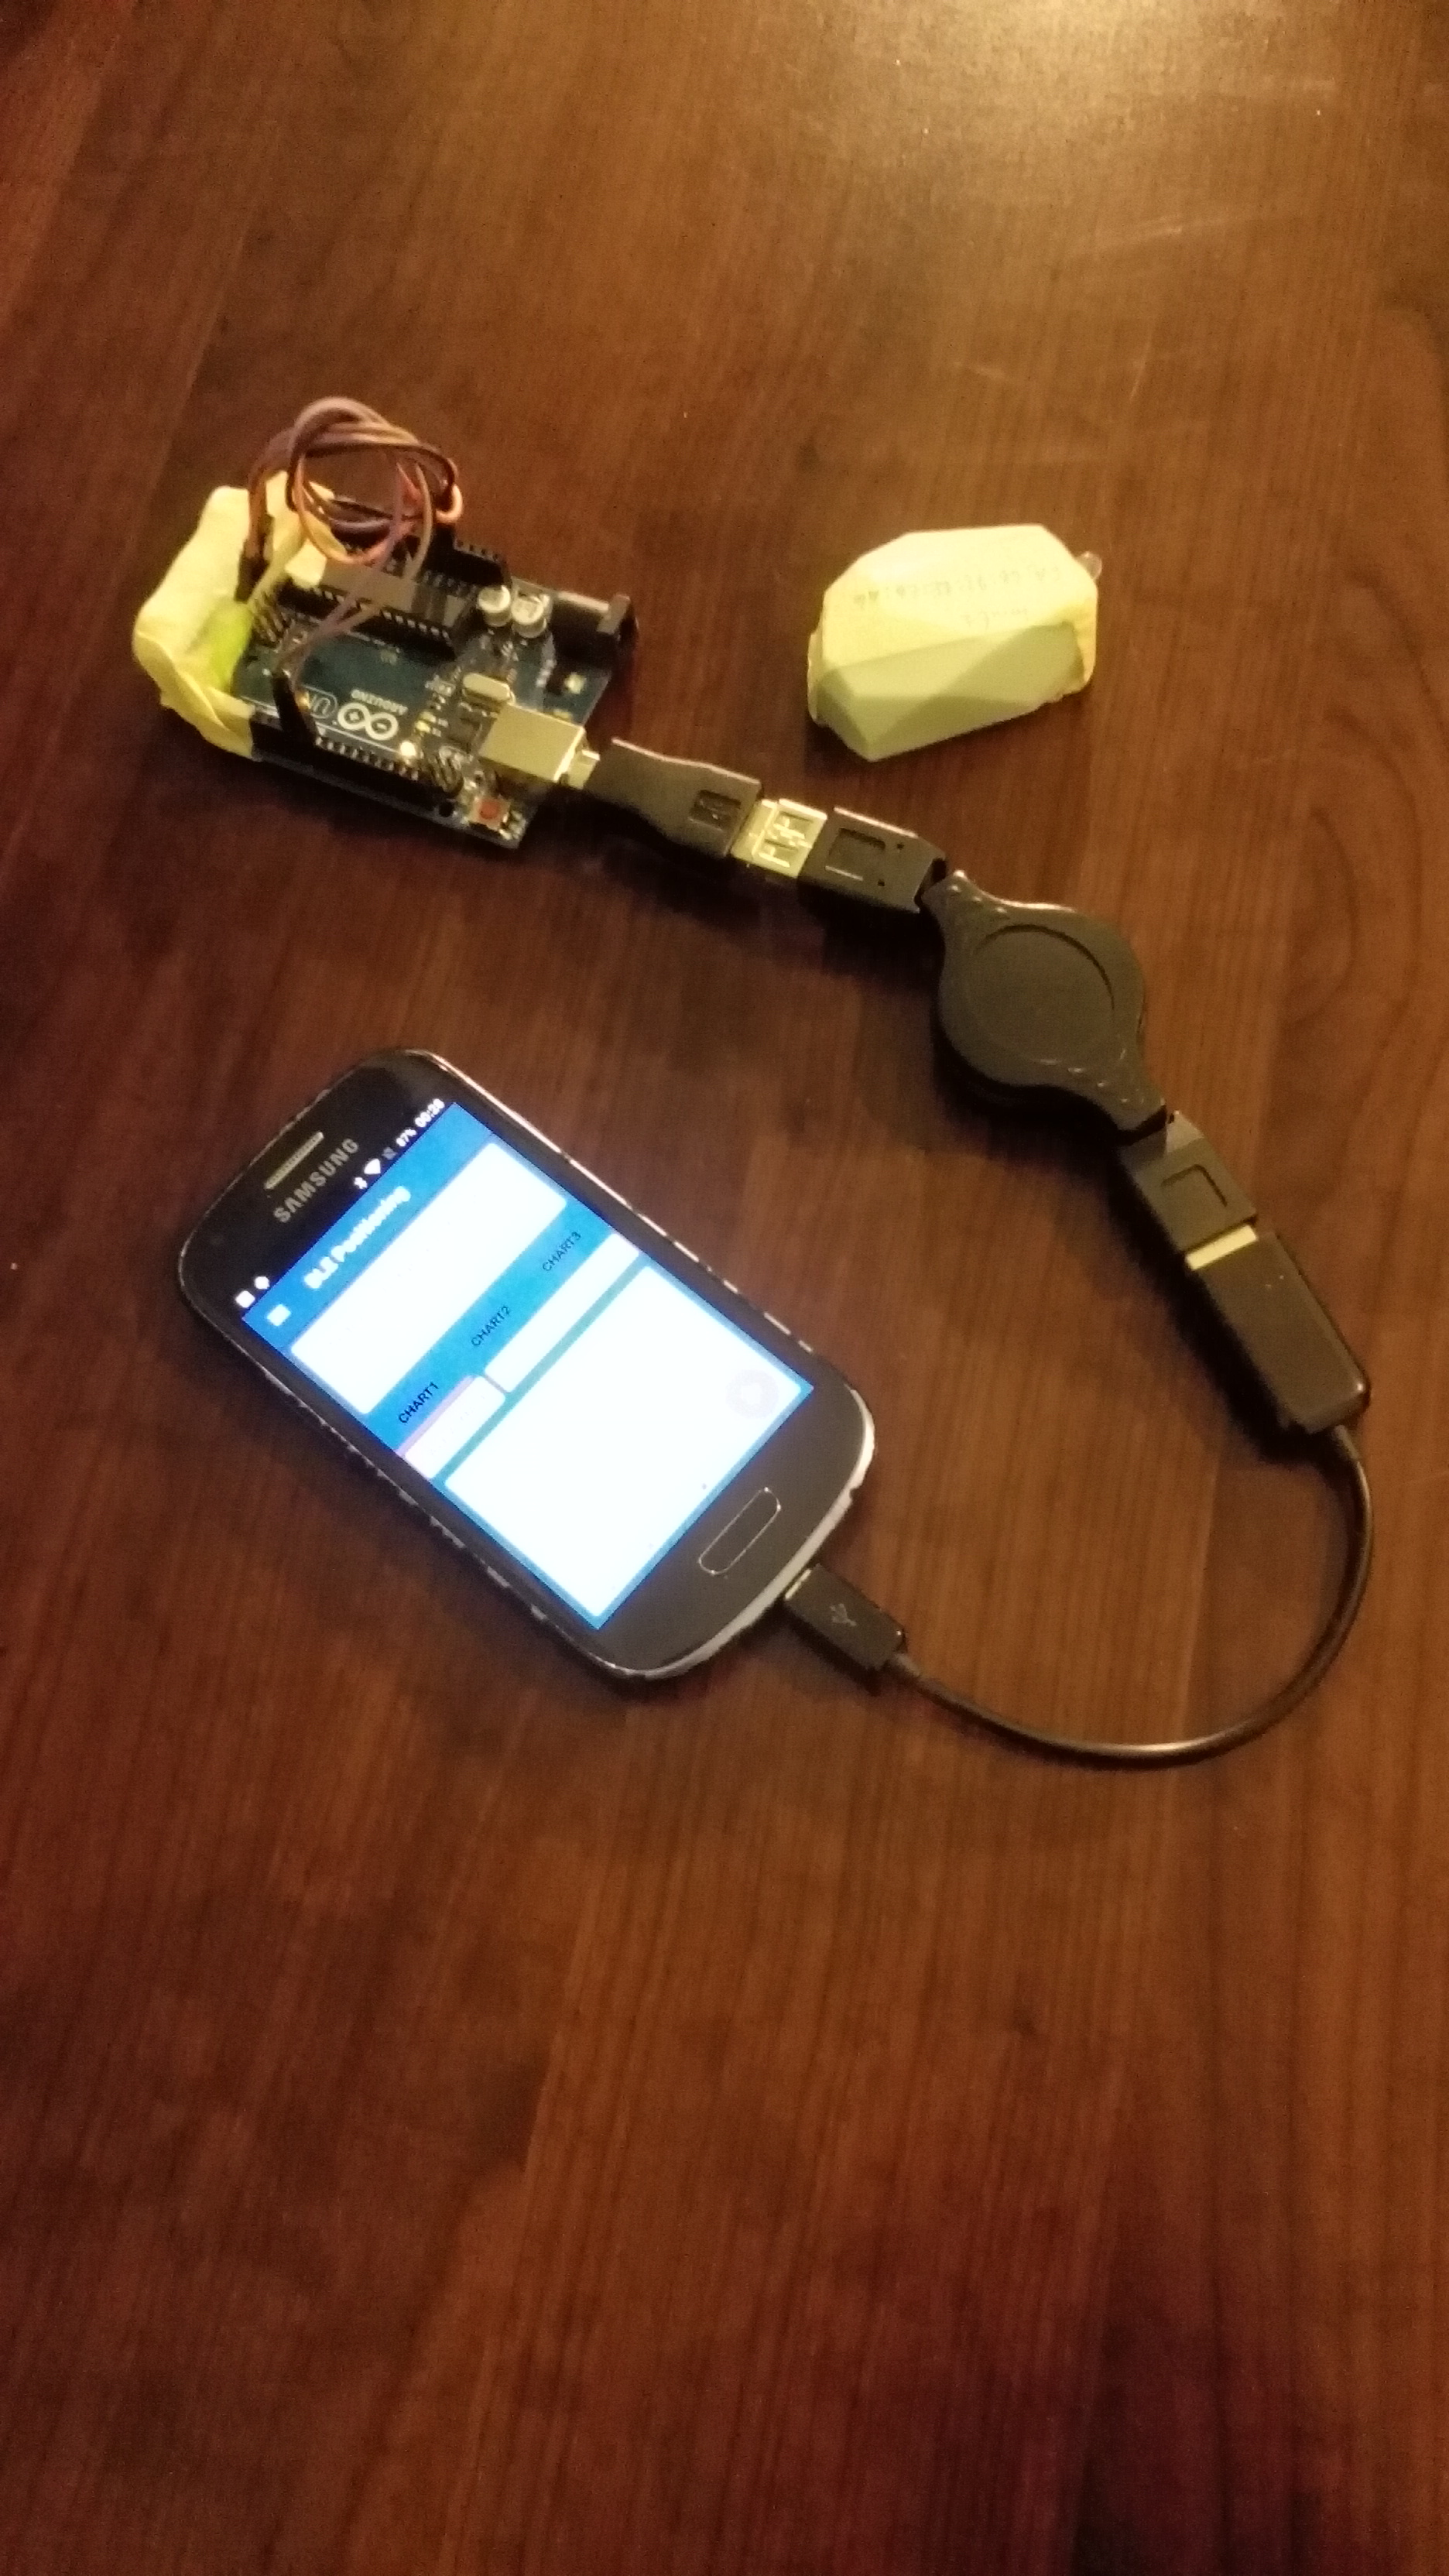
\includegraphics[width=0.3\linewidth]{img/otg/otg1.jpg}
	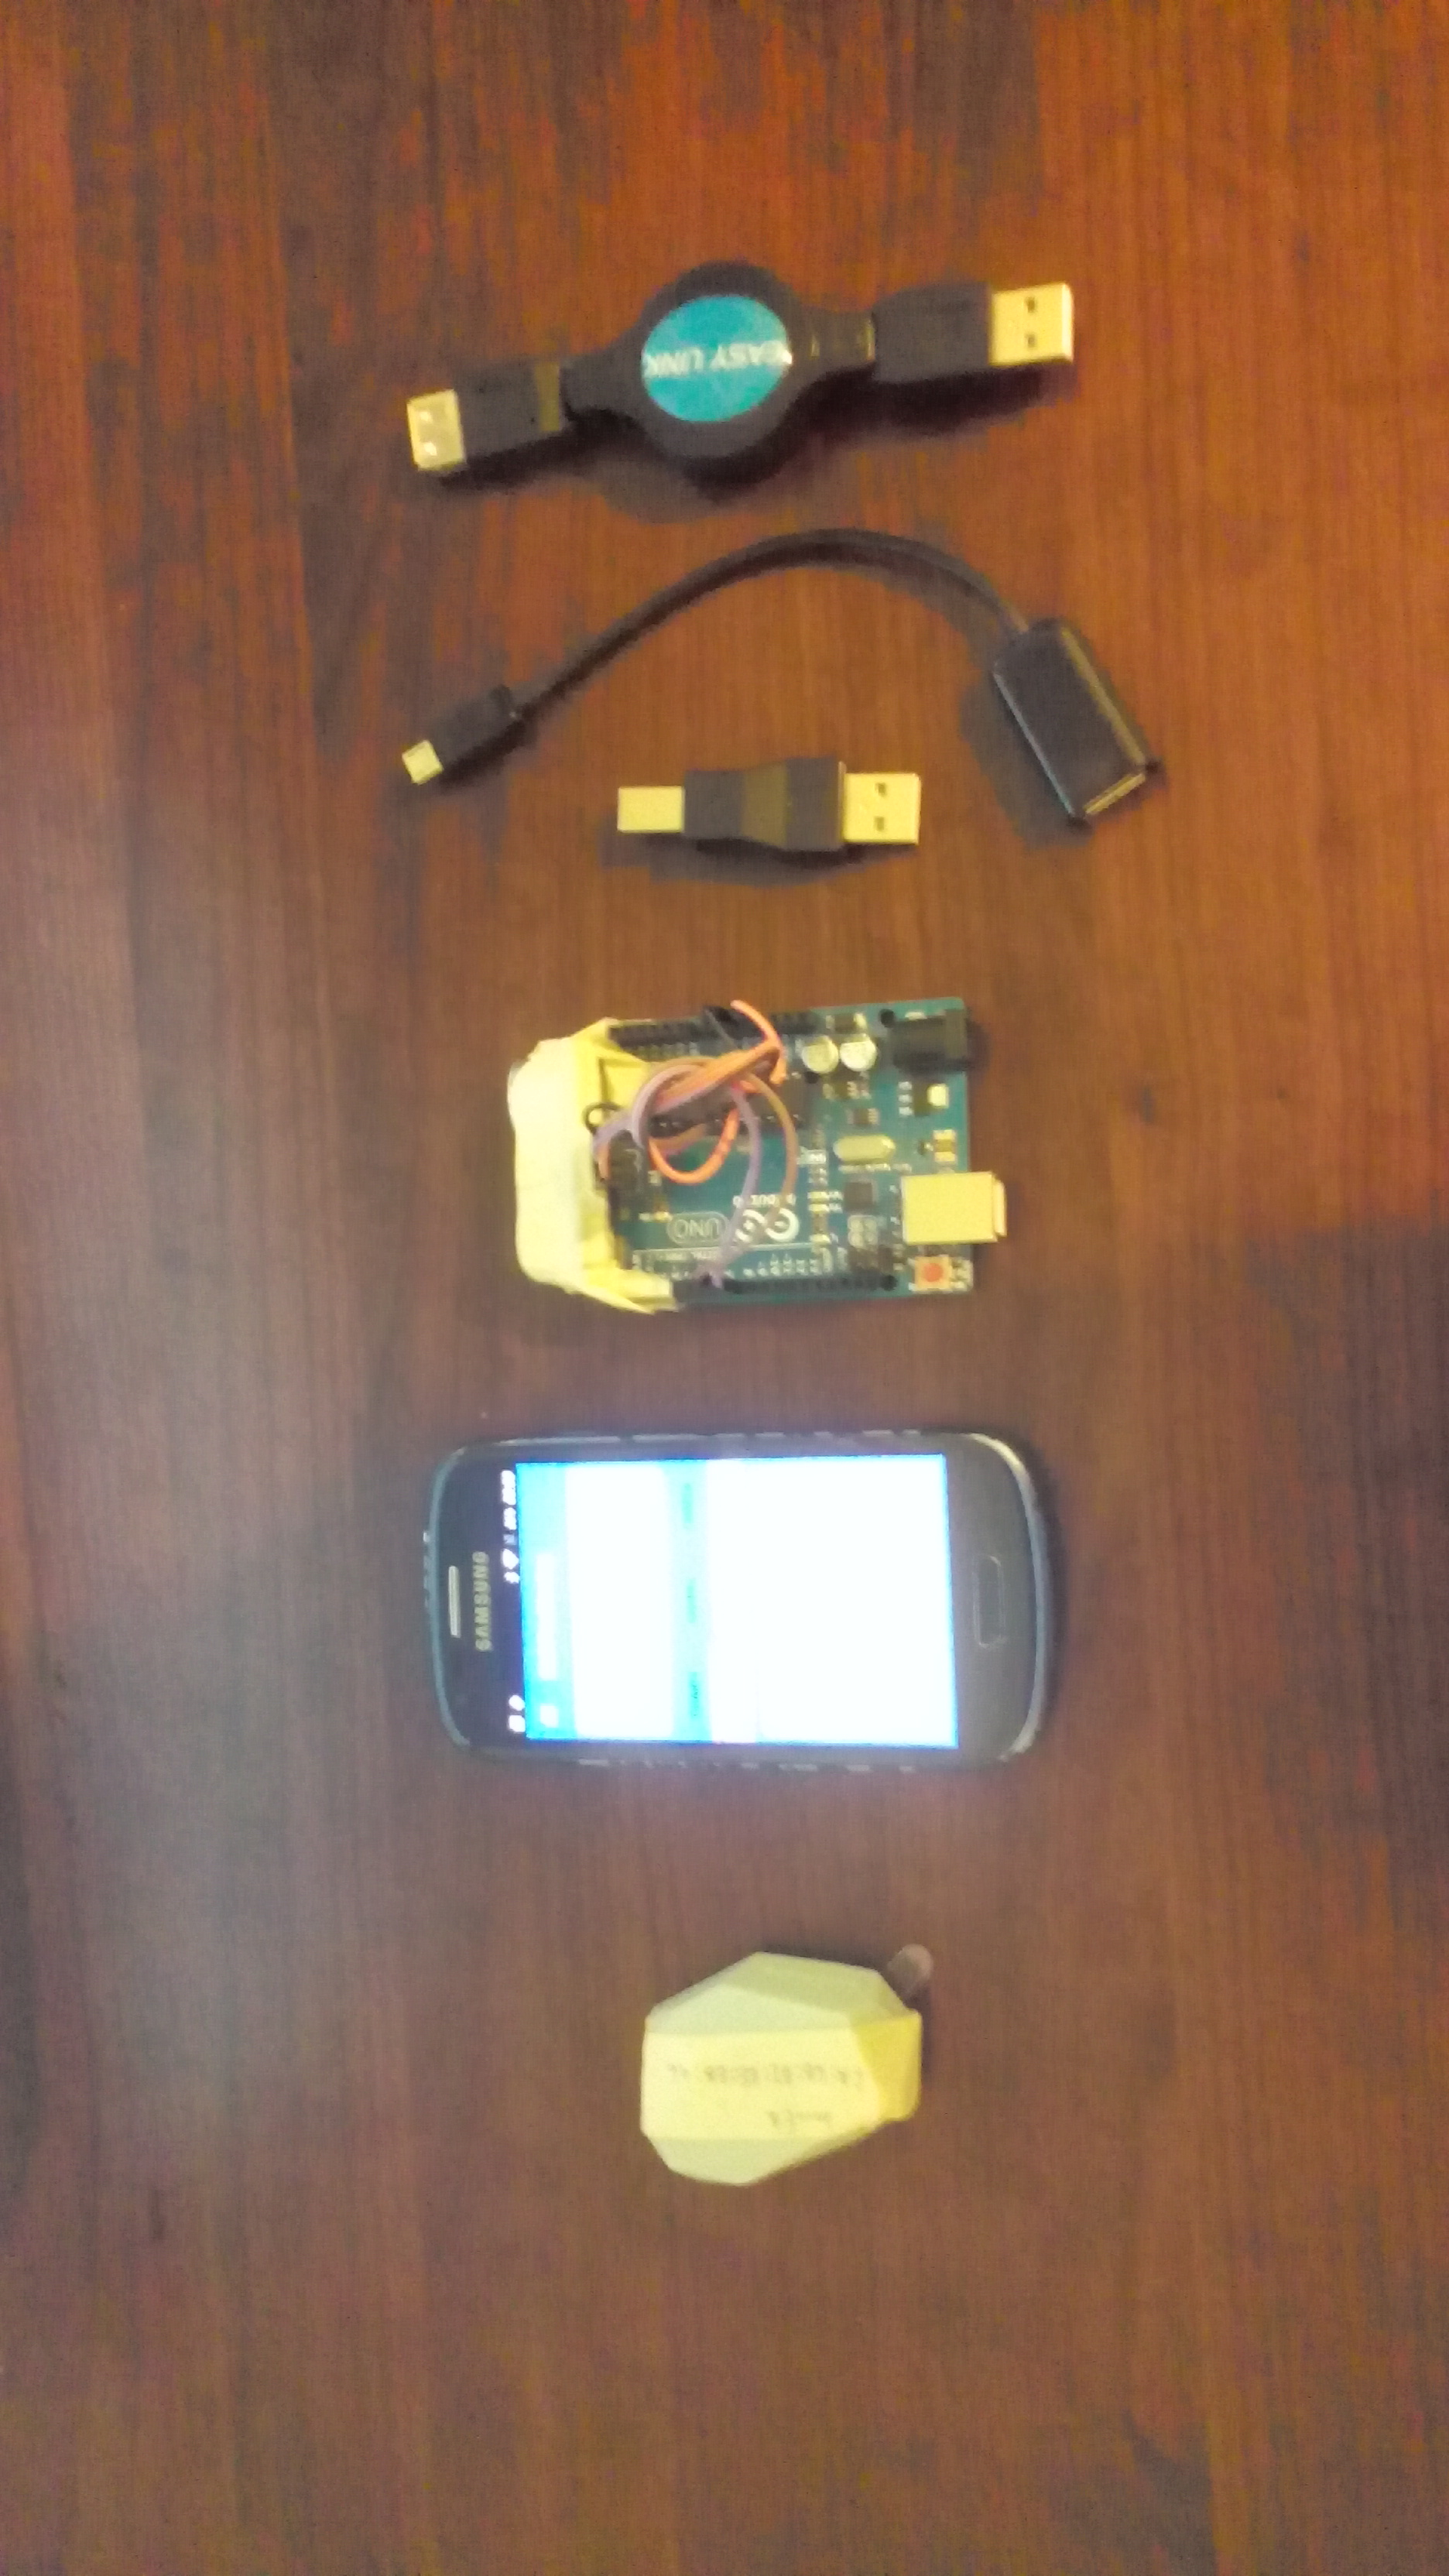
\includegraphics[width=0.3\linewidth]{img/otg/otg2.jpg}
	\caption{Collegamento Arduino-smartphone}
	\label{fig:collegamento_Arduino-smartphone}
\end{figure}

Questo approccio permette di avere un sensore di prossimità che restituisce una stima della distanza confrontabile con la stima eseguita con la tecnica RSSI.

\newpage
\subsection{Materiale utilizzato}
\begin{itemize}
	\item Samsung GT-I9190, \href{http://novafusion.pl/s3-mini/}{\textbf{CyanogenMod 12.1-20160718-UNOFFICIAL-golden Android 5.1.1}}\footnote{\href{http://novafusion.pl/s3-mini/}{\textbf{Novafusion}} - \url{http://novafusion.pl/s3-mini/}}.
	
	\item Sensore di prossimità ultrasonico HC-SR04.
	
	\item Cavo USB OTG ($ \sim 2$€).
	
\end{itemize}

\begin{figure}[ph]
	\centering
	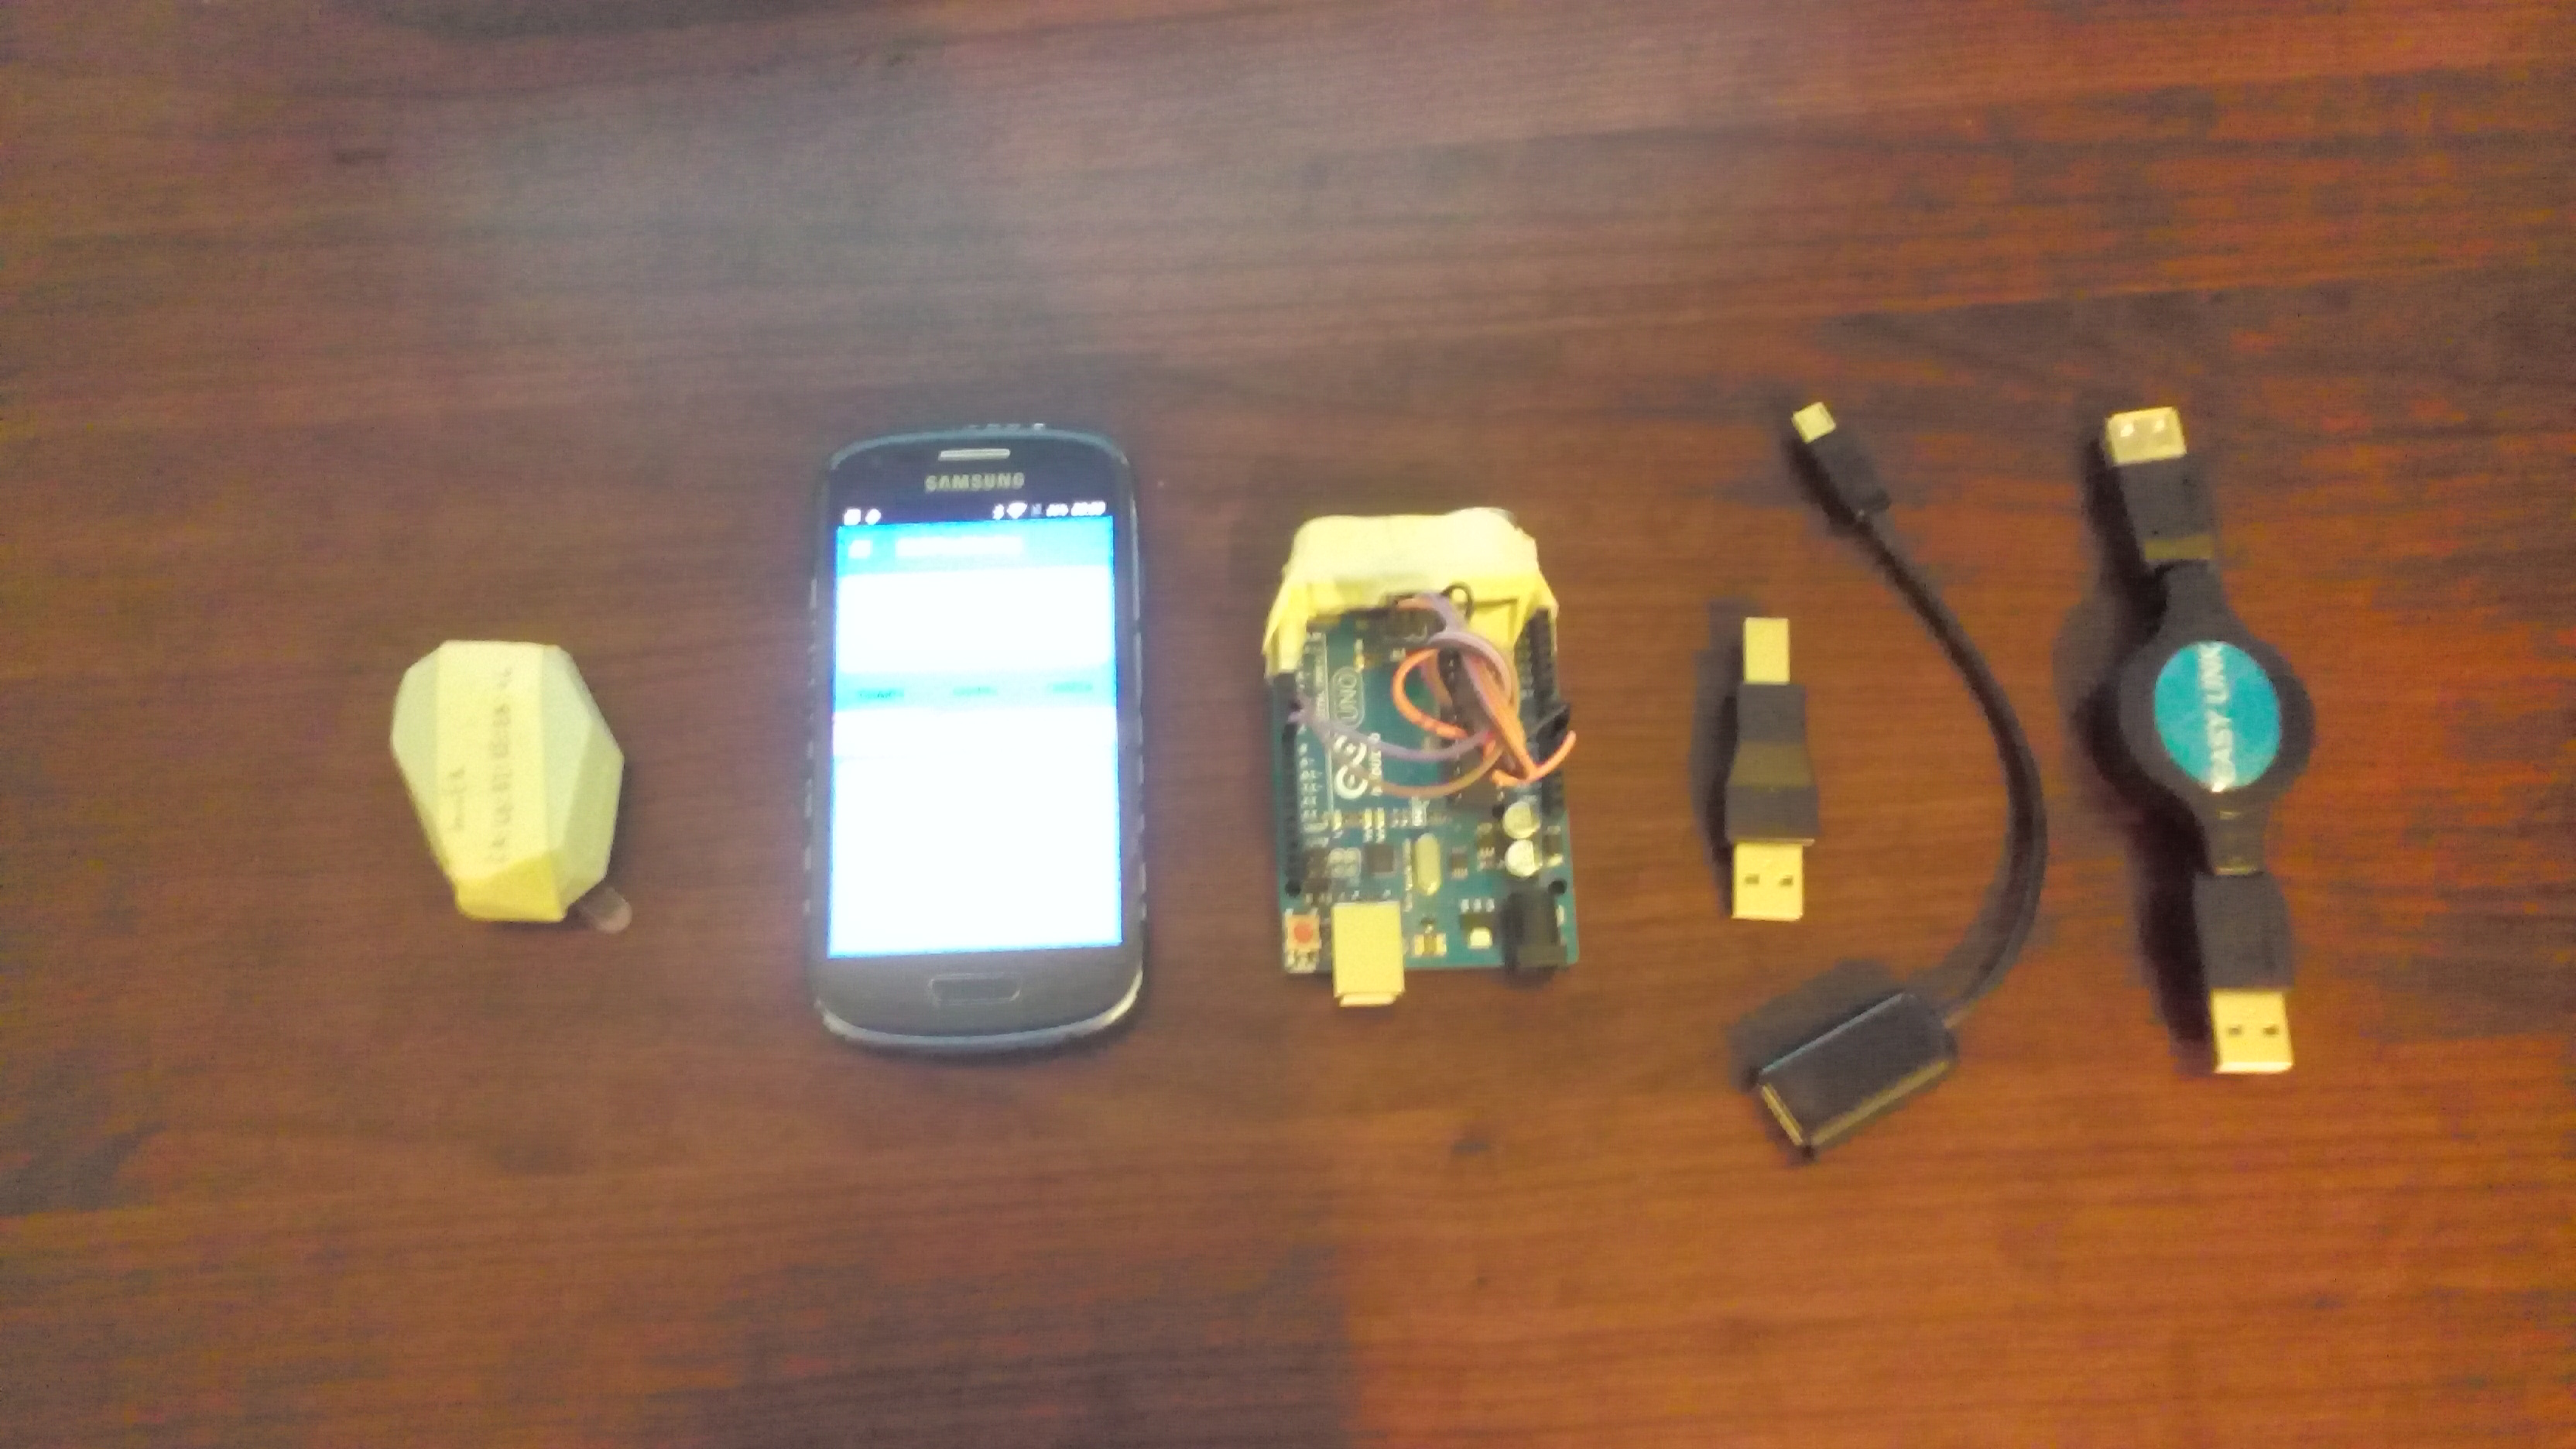
\includegraphics[width=0.8\linewidth]{img/otg/otg3.jpg}
	\caption{Materiale utilizzato}
\end{figure}

\chapter{Testing}

\section{Introduzione al testing}
Il testing è stato realizzato in una stanza che rispettava tutte le consegne indicate nel capitolo \ref{ch:preparazione_testing}.

Ogni rilevazione è durata esattamente 5 secondi. Ad ogni raccolta dati sono stati creati due file:
\begin{itemize}
	\item file \textit{.txt}: riassunto dei dati (data, ora, min, max e avg);
	\item file \textit{.json}: presenta tutti i dati raccolti e il loro riassunto in modo ben formattato.
\end{itemize} 
Questi file sono posti in cartelle e sottocartelle identificative all'interno del file system dello smartphone. Esempio di path: \texttt{/BLE Positioning Report/14-ott-2016/KF process noise 3.0/ARMA RSSI filter - Speed 0.1}

\section{Analisi dei dati raccolti}
Si è scelto di indicare solo i dati rilevanti al fine di evidenziare pregi e difetti della stima della distanza utilizzando tecnologie BLE.

Nei seguenti paragrafi è indicato il rumore di processo del filtro di Kalman considerato e le varie stime, dove:
\begin{itemize}
	\item \textbf{Raw}: indica la stima della distanza senza filtraggio;
	\item \textbf{AltBeacon}: è la stima della distanza built-in nella libreria AltBeacon;
	\item \textbf{Kalman Filter}: filtraggio dei dati Raw per migliorare la stima effettiva.
\end{itemize}

\section{Filtro Kalman con rumore di processo 1.0}
\subsection{No RSSI filtering}

In questo contesto si considera un rumore di processo posto ad 1.0,  ma senza imporre un filtraggio degli RSSI. Questo caso si considera come il \textbf{riferimento} da confrontare ad altre rilevazioni al fine di capire se utilizzare un filtro RSSI può aumentare l'accuratezza della stima.

La stima tende a diventare sempre meno precisa all'aumentare della distanza e dai 4 metri in poi diventa quasi impossibile riuscire ad avere una approssimazione degna di nota.

I casi peggiori per la stima considerata in questi test si registrano alla distanza di 3m. Nonostante questo il filtro di Kalman rispetto agli altri stimatori resta quello più fedele, anche se con un errore di circa mezzo metro.

Nei test riportati non sono considerati casi di utilizzo del filtro RunningAverageRssi in quanto con il suo impiego non sono state rilevate variazioni significative in positivo o negativo sulla stima della distanza.

\subsubsection{\underline{Riferimento ad 1m}}
\begin{center}
	\begin{tabular}{|c|c|c|c|c|c|c|}
		\hline 
		& \multicolumn{2}{|c|}{\textbf{Raw}} &\multicolumn{2}{|c|}{\textbf{AltBeacon}} &\multicolumn{2}{|c|}{\textbf{Kalman Filter}}\\ 
		\hline 
		& Stima (m) & Deviazione (m) & Stima (m) & Deviazione (m) & Stima (m)& Deviazione (m)\\ 
		\hline 
		\textbf{Min} & 1.01	& +0.01 & 0.97	& -0.03 & 1.00	& -0.00 \\ 
		\hline 
		\textbf{Max} & 1.11	& +0.11 & 1.01	& +0.01 & 1.00	& -0.00	\\ 
		\hline 
		\textbf{Avg} & 1.02	& +0.02 & 0.98 	& -0.02 & 1.00 	& -0.00	\\ 
		\hline 
	\end{tabular}
\end{center}

\newpage
\subsubsection{\underline{Riferimento ad 2m}}
\begin{center}
	\begin{tabular}{|c|c|c|c|c|c|c|}
		\hline 
		& \multicolumn{2}{|c|}{\textbf{Raw}} &\multicolumn{2}{|c|}{\textbf{AltBeacon}} &\multicolumn{2}{|c|}{\textbf{Kalman Filter}}\\ 
		\hline 
		& Stima (m) & Deviazione (m) & Stima (m) & Deviazione (m) & Stima (m)& Deviazione (m)\\ 
		\hline 
		\textbf{Min} & 1.22	& -0.78 & 1.06	& -0.94 & 1.91	& -0.09 \\ 
		\hline 
		\textbf{Max} & 1.92	& -0.08 & 1.34	& -0.66 & 2.09	& +0.09	\\ 
		\hline 
		\textbf{Avg} & 1.75	& -0.25 & 1.27 	& -0.73 & 2.04 	& +0.04	\\ 
		\hline 
	\end{tabular}
\end{center}

\subsubsection{\underline{Riferimento ad 3m}}
\begin{center}
	\begin{tabular}{|c|c|c|c|c|c|c|}
		\hline 
		& \multicolumn{2}{|c|}{\textbf{Raw}} &\multicolumn{2}{|c|}{\textbf{AltBeacon}} &\multicolumn{2}{|c|}{\textbf{Kalman Filter}}\\ 
		\hline 
		& Stima (m) & Deviazione (m) & Stima (m) & Deviazione (m) & Stima (m)& Deviazione (m)\\ 
		\hline 
		\textbf{Min} & 3.53	& +0.53 & 1.95	& -1.05 & 3.36	& +0.36 \\ 
		\hline 
		\textbf{Max} & 3.53	& +0.53 & 1.95	& -1.05 & 3.51	& +0.51	\\ 
		\hline 
		\textbf{Avg} & 3.53	& +0.53 & 1.95 	& -1.05 & 3.46 	& +0.46	\\ 
		\hline 
	\end{tabular}
\end{center}

Già da questi dati si evince che l'utilizzo del filtro di Kalman ha effettivamente migliorato la stima della distanza, soprattutto in confronto ad AltBeacon.

\newpage
\subsection{ARMA RSSI filter - Speed 0.1}

In questo contesto si considera sempre un rumore di processo 1.0,  ma oltre a questo si è applicato anche un filtro ARMA sugli RSSI.

L'obiettivo è verificare se l'utilizzo di questo filtro con lo speed a 0.1 aumenti la qualità della stima.

\subsubsection{\underline{Riferimento ad 1m}}
\begin{center}
	\begin{tabular}{|c|c|c|c|c|c|c|}
		\hline 
		& \multicolumn{2}{|c|}{\textbf{Raw}} &\multicolumn{2}{|c|}{\textbf{AltBeacon}} &\multicolumn{2}{|c|}{\textbf{Kalman Filter}}\\ 
		\hline 
		& Stima (m) & Deviazione (m) & Stima (m) & Deviazione (m) & Stima (m)& Deviazione (m)\\ 
		\hline 
		\textbf{Min} & 0.66	& -0.34 & 1.00	& -0.00 & 0.99	& -0.01 \\ 
		\hline 
		\textbf{Max} & 0.87	& -0.13 & 1.02	& +0.02 & 1.09	& +0.09	\\ 
		\hline 
		\textbf{Avg} & 0.78 	& -0.22 & 1.01 	& +0.01 & 1.04 	& +0.04	\\ 
		\hline 
	\end{tabular}
\end{center}

\subsubsection{\underline{Riferimento ad 2m}}
\begin{center}
	\begin{tabular}{|c|c|c|c|c|c|c|}
		\hline 
		& \multicolumn{2}{|c|}{\textbf{Raw}} &\multicolumn{2}{|c|}{\textbf{AltBeacon}} &\multicolumn{2}{|c|}{\textbf{Kalman Filter}}\\ 
		\hline 
		& Stima (m) & Deviazione (m) & Stima (m) & Deviazione (m) & Stima (m)& Deviazione (m)\\ 
		\hline 
		\textbf{Min} & 1.92	& -0.08 & 1.44	& -0.56 & 2.10	& +0.10 \\ 
		\hline 
		\textbf{Max} & 2.73	& +0.73 & 1.52	& -0.48 & 2.20	& +0.20	\\ 
		\hline 
		\textbf{Avg} & 2.14	& +0.14 & 1.47 	& -0.53 & 2.13 	& +0.13	\\ 
		\hline 
	\end{tabular}
\end{center}

\subsubsection{\underline{Riferimento ad 3m}}
\begin{center}
	\begin{tabular}{|c|c|c|c|c|c|c|}
		\hline 
		& \multicolumn{2}{|c|}{\textbf{Raw}} &\multicolumn{2}{|c|}{\textbf{AltBeacon}} &\multicolumn{2}{|c|}{\textbf{Kalman Filter}}\\ 
		\hline 
		& Stima (m) & Deviazione (m) & Stima (m) & Deviazione (m) & Stima (m)& Deviazione (m)\\ 
		\hline 
		\textbf{Min} & 2.73	& -0.27 & 1.70	& -1.30 & 2.77	& -0.23 \\ 
		\hline 
		\textbf{Max} & 4.18	& +0.08 & 1.75	& -1.25 & 3.07	& +0.07	\\ 
		\hline 
		\textbf{Avg} & 3.08	& +0.08 & 1.73 	& -1.27 & 2.86 	& -0.14	\\ 
		\hline 
	\end{tabular}
\end{center}

Dai dati ricavati emerge che l'utilizzo del filtro di Kalman con l'aggiunta di un filtro RSSI ha aumentato l'accuratezza della stima soprattutto nel caso peggiore. Nel dettaglio basta guardare la media che passa da un precedente +0.46m ad -0.14m per notare un sensibile miglioramento.

\newpage
\subsection{ARMA RSSI filter - Speed 0.25}

In questo test si è aumentato lo speed dell'ARMA filter per verificare se questo avesse qualche effetto positivo sul caso pessimo di stima.

\subsubsection{\underline{Riferimento ad 1m}}
\begin{center}
	\begin{tabular}{|c|c|c|c|c|c|c|}
		\hline 
		& \multicolumn{2}{|c|}{\textbf{Raw}} &\multicolumn{2}{|c|}{\textbf{AltBeacon}} &\multicolumn{2}{|c|}{\textbf{Kalman Filter}}\\ 
		\hline 
		& Stima (m) & Deviazione (m) & Stima (m) & Deviazione (m) & Stima (m)& Deviazione (m)\\ 
		\hline 
		\textbf{Min} & 0.87	& -0.13 & 0.93	& -0.07 & 1.08	& +0.08 \\ 
		\hline 
		\textbf{Max} & 0.87	& -0.13 & 10.98	& -0.02 & 1.19	& +0.19	\\ 
		\hline 
		\textbf{Avg} & 0.87 & -0.13 & 0.96 	& +0.04 & 1.14 	& +0.14	\\ 
		\hline 
	\end{tabular}
\end{center}

\subsubsection{\underline{Riferimento ad 2m}}
\begin{center}
	\begin{tabular}{|c|c|c|c|c|c|c|}
		\hline 
		& \multicolumn{2}{|c|}{\textbf{Raw}} &\multicolumn{2}{|c|}{\textbf{AltBeacon}} &\multicolumn{2}{|c|}{\textbf{Kalman Filter}}\\ 
		\hline 
		& Stima (m) & Deviazione (m) & Stima (m) & Deviazione (m) & Stima (m)& Deviazione (m)\\ 
		\hline 
		\textbf{Min} & 1.92	& -0.08 & 1.39	& -0.61 & 2.12	& +0.12 \\ 
		\hline 
		\textbf{Max} & 2.29	& +0.29 & 1.46	& -0.54 & 2.21	& +0.21	\\ 
		\hline 
		\textbf{Avg} & 2.12	& +0.12 & 1.42 	& -0.58 & 2.16 	& +0.16	\\ 
		\hline 
	\end{tabular}
\end{center}

\subsubsection{\underline{Riferimento ad 3m}}
\begin{center}
	\begin{tabular}{|c|c|c|c|c|c|c|}
		\hline 
		& \multicolumn{2}{|c|}{\textbf{Raw}} &\multicolumn{2}{|c|}{\textbf{AltBeacon}} &\multicolumn{2}{|c|}{\textbf{Kalman Filter}}\\ 
		\hline 
		& Stima (m) & Deviazione (m) & Stima (m) & Deviazione (m) & Stima (m)& Deviazione (m)\\ 
		\hline 
		\textbf{Min} & 3.84	& +0.84 & 2.27	& -0.73 & 3.61	& +0.61 \\ 
		\hline 
		\textbf{Max} & 4.93	& +1.20 & 2.35	& -0.65 & 3.86	& +0.86	\\ 
		\hline 
		\textbf{Avg} & 4.20	& +1.20 & 2.30 	& -0.70 & 3.79 	& +0.79	\\ 
		\hline 
	\end{tabular}
\end{center}

Dai dati raccolti sembra che all'aumentare dello speed non corrisponda un miglioramento, anzi sembra chiaro che ci sia una perdita di accuratezza, addirittura peggiore del caso senza filtraggio.

Questo comportamento è causato dal filtro ARMA il quale filtrando troppi pacchetti non permette di ottenere abbastanza informazioni RSSI, quindi le distanze stimate non sono più affidabili.

\newpage
\section{Filtro Kalman con rumore di processo 3.0}

In questi testi si considera un rumore di processo fissato a 3.0 per il filtro di Kalman e uno speed di 0.1 per il filtro ARMA.

\subsection{ARMA RSSI filter - Speed 0.1}

\subsubsection{\underline{Riferimento ad 1m}}
\begin{center}
	\begin{tabular}{|c|c|c|c|c|c|c|}
		\hline 
		& \multicolumn{2}{|c|}{\textbf{Raw}} &\multicolumn{2}{|c|}{\textbf{AltBeacon}} &\multicolumn{2}{|c|}{\textbf{Kalman Filter}}\\ 
		\hline 
		& Stima (m) & Deviazione (m) & Stima (m) & Deviazione (m) & Stima (m)& Deviazione (m)\\ 
		\hline 
		\textbf{Min} & 1.11	& +0.11 & 1.02	& +0.02 & 1.11	& +0.11 \\ 
		\hline 
		\textbf{Max} & 1.22	& +0.22 & 1.03	& +0.03 & 1.14	& +0.14	\\ 
		\hline 
		\textbf{Avg} & 1.12	& +0.12 & 1.02 	& +0.02 & 1.12 	& +0.12	\\ 
		\hline 
	\end{tabular}
\end{center}

\subsubsection{\underline{Riferimento ad 2m}}
\begin{center}
	\begin{tabular}{|c|c|c|c|c|c|c|}
		\hline 
		& \multicolumn{2}{|c|}{\textbf{Raw}} &\multicolumn{2}{|c|}{\textbf{AltBeacon}} &\multicolumn{2}{|c|}{\textbf{Kalman Filter}}\\ 
		\hline 
		& Stima (m) & Deviazione (m) & Stima (m) & Deviazione (m) & Stima (m)& Deviazione (m)\\ 
		\hline 
		\textbf{Min} & 2.29	& +0.29 & 1.48	& -0.52 & 2.19	& +0.19 \\ 
		\hline 
		\textbf{Max} & 2.73	& +0.73 & 1.52	& -0.48 & 2.23	& +0.23	\\ 
		\hline 
		\textbf{Avg} & 2.57	& +0.57 & 1.50 	& -0.50 & 2.20 	& +0.20	\\ 
		\hline 
	\end{tabular}
\end{center}

\subsubsection{\underline{Riferimento ad 3m}}
\begin{center}
	\begin{tabular}{|c|c|c|c|c|c|c|}
		\hline 
		& \multicolumn{2}{|c|}{\textbf{Raw}} &\multicolumn{2}{|c|}{\textbf{AltBeacon}} &\multicolumn{2}{|c|}{\textbf{Kalman Filter}}\\ 
		\hline 
		& Stima (m) & Deviazione (m) & Stima (m) & Deviazione (m) & Stima (m)& Deviazione (m)\\ 
		\hline 
		\textbf{Min} & 3.84	& +0.84 & 1.71	& -1.29 & 2.55	& -0.45 \\ 
		\hline 
		\textbf{Max} & 4.18	& +1.18 & 1.78	& -1.22 & 2.99	& -0.01	\\ 
		\hline 
		\textbf{Avg} & 4.11	& +1.11 & 1.74 	& -1.26 & 2.71 	& -0.29	\\ 
		\hline 
	\end{tabular}
\end{center}

Analizzando questi dati si comprende che questa configurazione presenta una stima migliore del caso senza filtro ARMA, ma peggiore di quella con il filtro di Kalman che ha meno rumore di processo.

L'effetto negativo (anche se contenuto), si deve al fatto che il filtro di Kalman con un valore troppo elevato di rumore di processo diventa più lento ed in generale restituisce dei valori RSSI che falsano la stima della distanza.

\newpage
\section{Conclusioni sui testing}
Dai test svolti si possono trarre le seguenti conclusioni:
\begin{enumerate}
	\item La scelta di fissare un tempo standard di rilevazione (5 secondi) ha permesso di confrontare più stime con diversi parametri di configurazione per ogni stimatore.
	\item L'utilizzo di Arduino durante la rilevazione delle distanze non è stata particolarmente agevole in quanto vi era sempre il rischio che questo inficiasse le rilevazioni.
	\item La libreria AltBeacon offre un metodo per stimare le distanze non particolarmente preciso, soprattutto oltre i 2 metri dal target.
	\item Il filtro di Kalman elimina gli \textit{spike} che si hanno nella rilevazione Raw.
	\item Il filtro di Kalman aumenta la precisione della stima delle distanze, soprattutto se si tara il rumore di processo nel modo giusto.
	\item I filtri Kalman e ARMA utilizzati insieme offrono una stima migliore, a patto che entrambi siano configurati nel modo giusto.	
\end{enumerate}

Una conclusione generale del progetto è che questo metodo di stima delle distanze, in base ai dati raccolti e agli strumenti usati, è ancora acerbo. L'utilizzo in campo proximity al momento sembra l'unico utilizzo reale in quanto superati i 3 metri la ricezione del segnale è altalenante, quindi la stima della distanza diventa troppo imprecisa.

Dai test svolti si è anche appreso che aggiungendo dei filtri (Kalman e ARMA) agli RSSI calcolati, la stima della distanza diventa più precisa; se a questi miglioramenti si potesse aggiungere una qualità/quantità della ricezione del segnale si otterrebbe una stima della distanza ancora più affidabile.